\chapter{आनुवंशिक अभियांत्रिकी और जैवप्रौद्योगिकी}\label{ch:b3:genetic-engineering}

1982 तक संसार का हर मधुमेही सूअरों और गोवंश के अग्न्याशयों से निकाले गए
इंसुलिन के सहारे जीवित रहता था --- एक किलोग्राम हॉर्मोन के लिए कोई आठ
हज़ार किलोग्राम ग्रंथियाँ --- और रोगियों का एक अंश उस पराए प्रोटीन के
विरुद्ध अनुक्रिया करता था। उसी वर्ष किसी आनुवंशिक रूप से अभियंत्रित जीव
से बनी पहली औषध बाज़ार में आई: मानव इंसुलिन, जिसे मानव जीन किसी
\omterm{def:b3:genetic-engineering:tools}{प्लाज़्मिड} पर ढोते \emph{Escherichia coli} ने संश्लेषित किया। जिन
औज़ारों ने यह संभव किया वे पिछले दशक में जुटाए गए थे --- ऐसे एंज़ाइम जो
DNA को चुने हुए अनुक्रमों पर काटते हैं, ऐसे एंज़ाइम जो टुकड़े जोड़ते
हैं, ऐसे \omterm{def:b3:genetic-engineering:tools}{प्लाज़्मिड} जो उन्हें किसी कोशिका में ले जाते और वहाँ उनकी नकल
करते हैं --- और अगले दशकों में उनमें \omterm{def:b3:genetic-engineering:pcr}{पॉलीमरेज़ शृंखला अभिक्रिया}, भ्रूणों
में जीनों का अंतःक्षेपण, और 2012 से कोई ऐसी जीवाणु प्रतिरक्षा-प्रणाली
जुड़ी जिसे क्रमादेश्य कैंची में बदल दिया गया है और जो किसी जीवित कोशिका
में जीनोम का एक अक्षर फिर से लिख सकती है। यह अध्याय उन्हीं औज़ारों के
बारे में है, उनके उपयोग को चलाने वाले अंकगणित के बारे में, और उनसे जो
बना है उसके बारे में --- किसी चमकते चूहे से लेकर दात्र-कोशिका रोग के
इलाज तक।

\section{DNA काटना, जोड़ना और नकल करना}

\begin{definition}[प्रतिबंधन एंज़ाइम, लाइगेज़ और संवाहक]\label{def:b3:genetic-engineering:tools}
\index{प्रतिबंधन एंज़ाइम}\index{चिपचिपा सिरा}\index{DNA लाइगेज़}\index{संवाहक}\index{प्लाज़्मिड}\index{वरणीय चिह्नक}
कोई प्रकार~II \emph{प्रतिबंधन एंज़ाइम} ऐसी जीवाणु एंडोन्यूक्लिएज़ है जो
द्विलड़ी DNA को \numrange{4}{8} क्षार युग्मों के किसी विशिष्ट अनुक्रम
पर काटती है, जो प्रायः कोई तालमेलक होता है: EcoRI G$^{\downarrow}$AATTC
काटती है और चार-क्षार की एकलड़ी अधिलंब (\emph{चिपचिपे सिरे}) छोड़ती है,
जो किसी भी दूसरे EcoRI सिरे के पूरक हैं; दूसरी एंज़ाइम \emph{भोथरे
सिरे} छोड़ती हैं। \emph{DNA लाइगेज़} ऐसे दो खंड जोड़ देती है जिनके सिरे
आपस में बैठते हों। कोई \emph{संवाहक} ऐसा DNA अणु है जो किसी परपोषी में
प्रतिकृत होता है और कोई अंतर्वेशित खंड ढो सकता है: कुछ किलोक्षारों का
कोई \emph{प्लाज़्मिड}, जिसमें प्रतिकृति का उद्गम, कोई
\emph{वरणीय चिह्नक} (कोई प्रतिजैविक-प्रतिरोध जीन, ताकि प्रतिजैविक पर
केवल वही कोशिकाएँ उगें जिन्होंने प्लाज़्मिड लिया) और अंतर्वेशन के लिए
अनन्य प्रतिबंधन स्थलों का एक गुच्छा हो; जीवाणुभोजी $\lambda$, कॉस्मिड,
और \qtyrange{20}{1000}{kb} के अंतर्वेशनों के लिए जीवाणु अथवा खमीर के
कृत्रिम गुणसूत्र। DNA किसी जीवाणु में \emph{रूपांतरण} से घुसता है, किसी
ऐसे रासायनिक या वैद्युत आघात के बाद जो झिल्ली को क्षण भर के लिए पारगम्य
बना देता है, और दक्षता प्रति माइक्रोग्राम प्लाज़्मिड $10^{6}$ से $10^{9}$
रूपांतरित कोशिकाएँ होती है। कोई \emph{पुनर्योगज} अणु वह है जो दो
स्रोतों का DNA जोड़ता है।
\end{definition}

\begin{proof}[प्रमाण-सामग्री]
कोहेन, चांग, बॉयर और हेलिंग (1973) ने \omterm{def:b3:genetic-engineering:tools}{प्लाज़्मिड} pSC101 और किसी दूसरे
प्रतिरोध जीन वाले दूसरे \omterm{def:b3:genetic-engineering:tools}{प्लाज़्मिड} को EcoRI से काटा, खंडों को मिलाकर
जोड़ा, \emph{E.~coli} का रूपांतरण किया, और ऐसी बस्तियाँ पाईं जो दोनों
प्रतिजैविकों के प्रति प्रतिरोधी थीं और दोनों से बना एक ही \omterm{def:b3:genetic-engineering:tools}{प्लाज़्मिड} ढो
रही थीं --- किसी कोशिका में प्रतिकृत होने वाला पहला पुनर्योगज DNA। अगले
वर्ष उन्होंने किसी भेक के राइबोसोमी RNA जीन pSC101 में डाले और दिखाया कि
मेंढक का DNA जीवाणु में प्रतिकृत भी हुआ और अनुलेखित भी: जीन जगतों की
सीमा बिना बदले पार करते हैं, और कोई जीवाणु उसे दिया गया कोई भी DNA नकल
कर देगा।
\end{proof}

\begin{omfigure}
\begin{tikzpicture}[every node/.style={font=\scriptsize}, >=stealth]
  % plasmid circle
  \draw[very thick, omDef] (0,0) circle (1.8);
  % ori
  \draw[very thick, omMeth!70!black] (0,0) ++(60:1.8) arc[start angle=60, end angle=100, radius=1.8]; \node[above right] at (80:1.95) {प्रतिकृति का उद्गम};
  % ampR
  \draw[very thick, omProp] (0,0) ++(160:1.8) arc[start angle=160, end angle=250, radius=1.8]; \node[left, align=right] at (205:2.0) {प्रतिरोध\\जीन (चिह्नक)};
  % MCS with insert
  \draw[very thick, omThm] (0,0) ++(-40:1.8) arc[start angle=-40, end angle=10, radius=1.8]; \node[right, align=left] at (-15:2.0) {अंतर्वेशन, प्रतिबंधन स्थल\\में जोड़ा गया};
  \draw[omThm] (-40:1.7) -- (-40:1.95); \draw[omThm] (10:1.7) -- (10:1.95);
  \node at (0,0.25) {प्लाज़्मिड}; \node at (0,-0.15) {\qtyrange{3}{5}{kb}};
  % sticky ends detail
  \begin{scope}[xshift=5.7cm, yshift=0.8cm]
    \node[left, align=right] at (-0.2,0) {EcoRI};
    \node[font=\ttfamily\scriptsize, anchor=west] at (0,0.25) {5$'$-G\,\textcolor{omThm}{AATT}C-3$'$};
    \node[font=\ttfamily\scriptsize, anchor=west] at (0,-0.25) {3$'$-C\textcolor{omThm}{TTAA}\,G-5$'$};
    \draw[->, omThm, thick] (0.62,0.55) -- (0.62,0.3); \draw[->, omThm, thick] (1.62,-0.55) -- (1.62,-0.3);
    \node[anchor=west, align=left] at (2.9,0) {विषम कटाव पूरक चार-क्षार\\अधिलंब छोड़ते हैं:\\चिपचिपे सिरे};
  \end{scope}
  \begin{scope}[xshift=5.7cm, yshift=-1.3cm]
    \draw[very thick, omDef] (0,0.15) -- (1.2,0.15); \draw[very thick, omDef] (0,-0.15) -- (0.7,-0.15);
    \draw[very thick, omThm] (1.7,0.15) -- (3.0,0.15); \draw[very thick, omThm] (1.2,-0.15) -- (3.0,-0.15);
    \node[above] at (1.45,0.2) {तापानुशीतन}; \node[below, align=center] at (1.5,-0.25) {कोई भी दो EcoRI सिरे युग्मित होते हैं;\\लाइगेज़ आधार-ढाँचा जोड़ देती है};
  \end{scope}
\end{tikzpicture}

{\small कोई क्लोनन \omterm{def:b3:genetic-engineering:tools}{संवाहक} और उसकी रसायन। \omterm{def:b3:genetic-engineering:tools}{प्लाज़्मिड} एक उद्गम, एक
\omterm{def:b3:genetic-engineering:tools}{वरणीय चिह्नक} और एक अनन्य प्रतिबंधन स्थल ढोता है, जिसमें उसी एंज़ाइम से
कटा कोई खंड जोड़ा जाता है; चिपचिपे सिरे एक ही एंज़ाइम से कटे किन्हीं भी
दो खंडों को संगत बना देते हैं।}
\end{omfigure}

\begin{method}[किसी जीन का क्लोनन]\label{met:b3:genetic-engineering:cloning}
\index{क्लोनन}\index{संचय}\index{छानबीन}
(1) अंतर्वेशन पाइए: जीनोमी DNA को किसी \omterm{def:b3:genetic-engineering:tools}{प्रतिबंधन एंज़ाइम} से काटिए, या
संदेशवाहक RNA की नकल पूरक DNA (cDNA, जिसमें अंतर्वेशन नहीं होते और
इसलिए जिसे जीवाणुओं में अभिव्यक्त किया जा सकता है) में कीजिए, या
प्रतिबंधन स्थल ढोते \omterm{def:b3:genetic-engineering:pcr}{प्रारंभकों} से जीन को PCR द्वारा प्रवर्धित कीजिए।
(2) \omterm{def:b3:genetic-engineering:tools}{संवाहक} और अंतर्वेशन को एक ही एंज़ाइम (या एंज़ाइमों) से काटिए ---
दो भिन्न एंज़ाइम अंतर्वेशन की दिशा बाध्य कर देते हैं --- और जोड़िए।
(3) जीवाणुओं का रूपांतरण कीजिए और प्रतिजैविक पर फैलाइए: केवल वही
कोशिकाएँ उगती हैं जिनमें कोई \omterm{def:b3:genetic-engineering:tools}{प्लाज़्मिड} है। (4) अंतर्वेशन वाले
\omterm{def:b3:genetic-engineering:tools}{प्लाज़्मिडों} को उनसे अलग कीजिए जो स्वयं पर ही बंद हो गए: क्लोनन स्थल
से टूटा कोई चिह्नक जीन (\emph{lacZ}: सफ़ेद बस्तियों में अंतर्वेशन है,
नीली में नहीं)। (5) वांछित अंतर्वेशन के लिए बस्तियों की छानबीन कीजिए:
किसी अंकित अन्वेषी से संकरण द्वारा, PCR से, या प्रतिबंधन पाचन तथा जेल
वैद्युत-कणसंचलन से। (6) अंतर्वेशन का अनुक्रमण कीजिए। कोई \emph{संचय}
किसी पूरे जीनोम या अनुलेखितांश के क्लोनों का समूह है, जिसमें से उसी
छानबीन द्वारा कोई भी जीन निकाला जा सकता है।
\end{method}

\begin{omfigure}
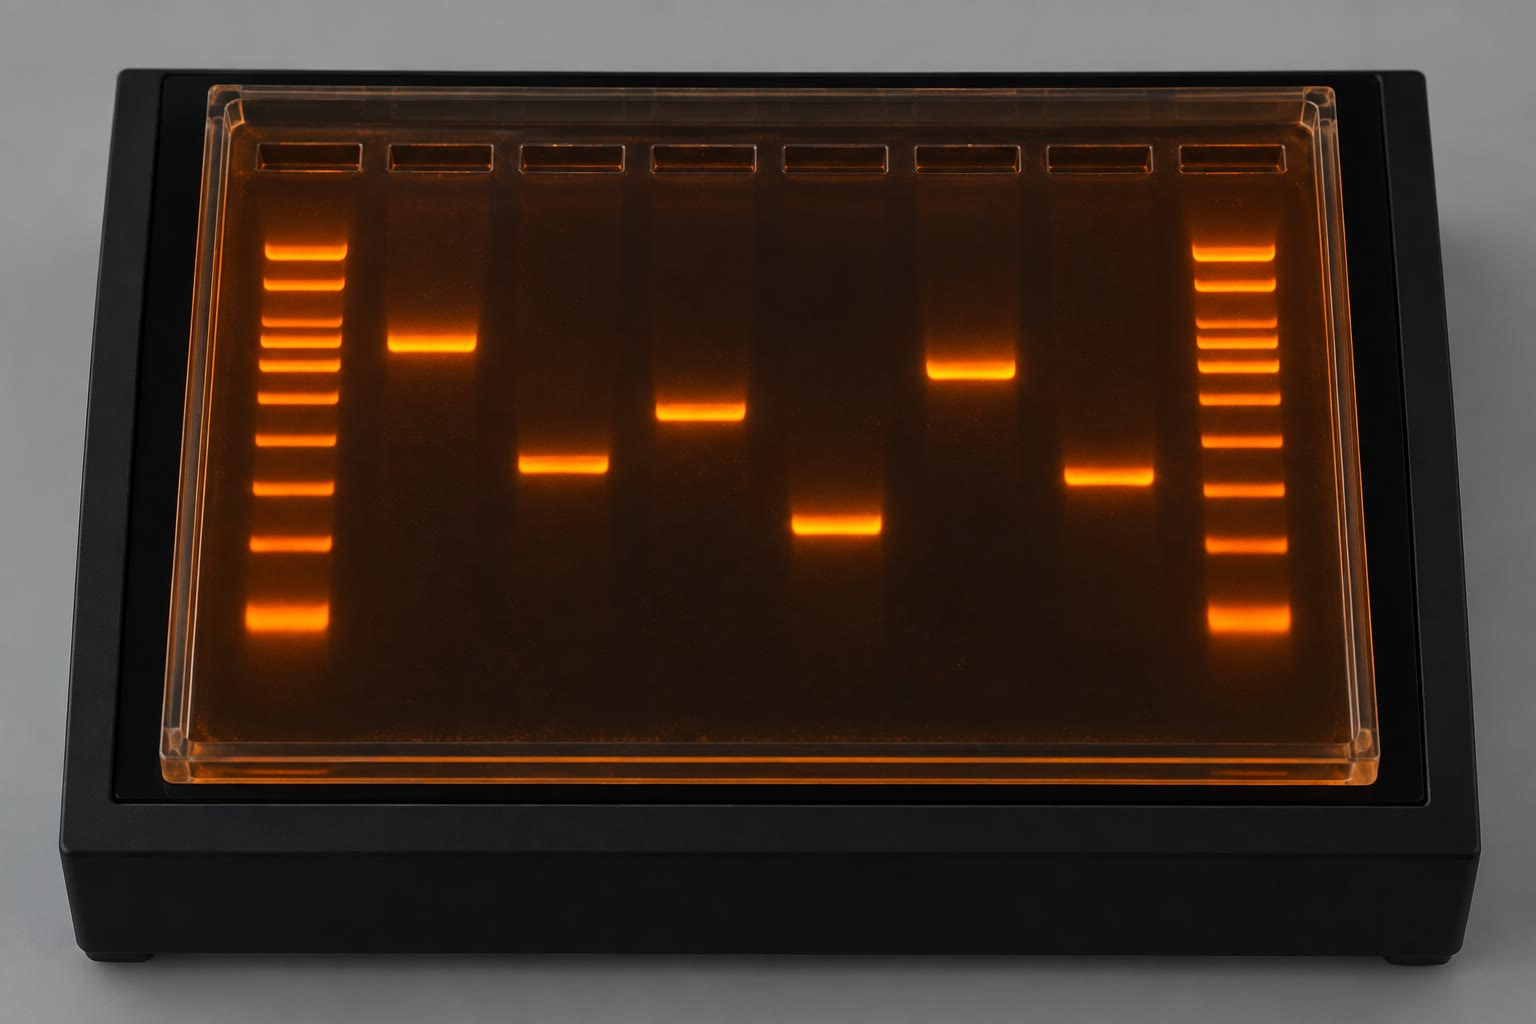
\includegraphics[width=0.56\linewidth]{images/book5/ai/b5-06-agarose-gel.jpg}

{\small पराबैंगनी प्रकाश के नीचे कोई ऐगरोज़ जेल: DNA खंड धनाग्र की ओर
ऐसी चाल से चलते हैं जो उनकी लंबाई के साथ गिरती है, इसलिए हर पट्टी एक ही
आकार के अणुओं की समष्टि है, जिसकी तुलना बाहरी पथों में ज्ञात आकारों की
सीढ़ी से की जाती है।}
\end{omfigure}

\begin{definition}[पॉलीमरेज़ शृंखला अभिक्रिया]\label{def:b3:genetic-engineering:pcr}
\index{पॉलीमरेज़ शृंखला अभिक्रिया}\index{प्रारंभक}\index{मात्रात्मक PCR}
\emph{पॉलीमरेज़ शृंखला अभिक्रिया} (PCR) दो \emph{प्रारंभकों} के बीच के
किसी चुने हुए DNA खंड को प्रवर्धित करती है --- प्रारंभक लगभग बीस
क्षारों के संश्लेषित ऑलिगोन्यूक्लियोटाइड हैं जो लक्ष्य के सिरों पर
दोनों लड़ियों के पूरक हैं --- तीन तापों के चक्रों के द्वारा:
लड़ियाँ अलग करने के लिए \qty{95}{\celsius}, प्रारंभकों के तापानुशीतन के
लिए \qtyrange{50}{65}{\celsius}, और किसी ताप-स्थायी पॉलीमरेज़ (Taq, जो
गर्म-सोते के जीवाणु \emph{Thermus aquaticus} से आती है) द्वारा उन्हें
बढ़ाने के लिए \qty{72}{\celsius}। हर चक्र प्रारंभकों के बीच के खंड की
प्रतियों की संख्या दोगुनी कर देता है, इसलिए तीस चक्र एक अकेले अणु को
एक अरब बना देते हैं। \emph{प्रतिलोम अनुलेखन PCR} पहले RNA की नकल DNA
में करती है और इस तरह अनुलेखों या RNA विषाणुओं को मापती है;
\emph{मात्रात्मक PCR} (qPCR) प्रवर्धन को वास्तविक समय में किसी
प्रतिदीप्त रंजक से देखती है और आरंभिक मात्रा उस चक्र से पढ़ लेती है
जिस पर संकेत किसी देहली को पार करता है।
\end{definition}

\begin{theorem}[प्रवर्धन का अंकगणित]\label{thm:b3:genetic-engineering:pcr}
\index{देहली चक्र}
प्रति चक्र दक्षता $E$ के साथ (पूर्ण द्विगुणन के लिए $E = 1$), $N_{0}$
आरंभिक प्रतियाँ बन जाती हैं
\[
N_{n} = N_{0}\,(1 + E)^{n}
\]
$n$ चक्रों के बाद। यदि प्रतिदीप्ति किसी नियत देहली को तब पार करे जब
प्रति-संख्या $N_{T}$ तक पहुँचे, तो \emph{\omterm{thm:b3:genetic-engineering:pcr}{देहली चक्र}} है
\[
C_{T} = \frac{\log N_{T} - \log N_{0}}{\log(1 + E)},
\]
जो $\log N_{0}$ में ढाल $-1/\log(1+E)$ वाली एक सरल रेखा है: $E = 1$ के
लिए, आरंभिक मात्रा में हर दस गुना वृद्धि $C_{T}$ को
$\log_{2} 10 = 3.32$ चक्र नीचे ले आती है, और जिन दो प्रतिदर्शों के
\omterm{thm:b3:genetic-engineering:pcr}{देहली चक्र} $\Delta C_{T}$ से भिन्न हों उनकी आरंभिक प्रतियों में गुणक
$(1 + E)^{\Delta C_{T}}$ का अंतर होता है।
\end{theorem}
\begin{proof}
हर चक्र प्रति-संख्या को $1 + E$ से गुणा करता है, इसलिए $N_{n}$ कोई
गुणोत्तर अनुक्रम है। $N_{n} = N_{T}$ रखकर $n$ के लिए हल करने पर
$C_{T}$ मिलता है; ढाल $\log N_{0}$ का गुणांक है। दो प्रतिदर्शों के लिए
$C_{T,1} - C_{T,2} = (\log N_{0,2} - \log N_{0,1})/\log(1+E)$, जिससे
$N_{0,2}/N_{0,1} = (1+E)^{\Delta C_{T}}$।
\end{proof}

\begin{example}[कोई qPCR पट्टिका पढ़ना]\label{ex:b3:genetic-engineering:qpcr}
कोई विषाणु-RNA परीक्षण एक रोगी के लिए चक्र $22$ पर और दूसरे के लिए
चक्र $32$ पर देहली पार करता है; $E \approx 1$ के साथ पहले में $2^{10}
\approx 1000$ गुना अधिक विषाणु है। दस प्रतियों वाला कोई प्रतिदर्श लगभग
चक्र $37$ पर पार करता है जब देहली $10^{12}$ प्रतियाँ हो ($\log_{2} 10^{11} =
36.5$); इसलिए $40$ चक्रों की कोई बारी कुछ ही अणु पकड़ लेती है, और किसी
पिछले प्रवर्धित उत्पाद का एक अकेला संदूषक अणु भी पकड़ा जाता है, यही
कारण है कि प्रयोगशालाएँ PCR लगाने के कमरे उन कमरों से अलग रखती हैं जहाँ
उत्पाद सँभाले जाते हैं।
\end{example}

\begin{omfigure}
\begin{tikzpicture}
\begin{axis}[
  width=0.7\linewidth, height=5.6cm,
  axis x line=bottom, axis y line=left,
  xmin=0, xmax=40, ymin=1, ymax=1e14, ymode=log,
  xlabel={चक्र}, ylabel={प्रतियाँ},
  xlabel style={font=\small, at={(axis description cs:0.5,-0.12)}, anchor=north},
  ylabel style={font=\small},
  tick label style={font=\small}, xtick={0,10,20,30,40},
  clip=false,
]
\addplot[very thick, omDef, domain=0:40, samples=41] {1e7*2^x/(1+2^x/1e5)};
\addplot[very thick, omThm, domain=0:40, samples=41] {1e4*2^x/(1+2^x/1e8)};
\addplot[very thick, omMeth!70!black, domain=0:40, samples=41] {10*2^x/(1+2^x/1e11)};
\addplot[dashed, gray, domain=0:40, samples=2] {1e12};
\node[font=\scriptsize, gray, anchor=south west] at (axis cs:0.5,1.3e12) {देहली $N_{T}$};
\draw[gray] (axis cs:16.6,1) -- (axis cs:16.6,1e12); \draw[gray] (axis cs:26.6,1) -- (axis cs:26.6,1e12); \draw[gray] (axis cs:36.5,1) -- (axis cs:36.5,1e12);
\node[font=\scriptsize, anchor=south] at (axis cs:16.6,3e12) {$C_{T} = 16.6$}; \node[font=\scriptsize, anchor=south] at (axis cs:26.6,3e12) {$26.6$}; \node[font=\scriptsize, anchor=south] at (axis cs:36.5,3e12) {$36.5$};
\end{axis}
\end{tikzpicture}

{\small $N_{0} = 10^{7}$ (नीला), $10^{4}$ (लाल)
और $10$ प्रतियों (हरा) के लिए प्रवर्धन-वक्र, $E = 1$, और वह पठार जो अभिकर्मक थोप देते हैं।
$N_{0}$ में हज़ार गुना अंतर \omterm{thm:b3:genetic-engineering:pcr}{देहली चक्र} को $10$ खिसका देता है; पठार सब
एक जैसे हैं, इसीलिए अंतिम उत्पाद आरंभ के बारे में कुछ नहीं बताता।}
\end{omfigure}

\section{प्रोटीन बनाना}

\begin{definition}[अभिव्यक्ति प्रणालियाँ]\label{def:b3:genetic-engineering:expression}
\index{अभिव्यक्ति संवाहक}\index{पुनर्योगज प्रोटीन}\index{एकक्लोनी प्रतिरक्षी}
कोई \emph{अभिव्यक्ति \omterm{def:b3:genetic-engineering:tools}{संवाहक}} क्लोनित कूटलेखी अनुक्रम को परपोषी के किसी
प्रबल, नियंत्रणीय प्रवर्तक के अधीन रखता है (\emph{E.~coli} में
\emph{lac} या T7 प्रवर्तक, जो किसी शर्करा-अनुरूप से प्रेरित होता है),
साथ में कोई राइबोसोम-बंधक स्थल, कोई समापक, और प्रायः कोई \emph{अनुलग्नक}
--- छह हिस्टिडीन, कोई छोटा प्रोटीन --- जो स्तंभ पर शुद्धीकरण के लिए
उत्पाद से संलयित होता है। जीवाणु किसी सरल प्रोटीन (इंसुलिन,
वृद्धि हॉर्मोन, एंज़ाइम) के प्रति लीटर ग्राम बना देते हैं पर जटिल
स्तनधारी प्रोटीनों का ग्लाइकोसिलीकरण या वलन नहीं कर सकते; खमीर अपनी ही
तरह की शर्कराएँ जोड़ता है; कीट और स्तनधारी कोशिकाएँ (चीनी हैम्स्टर
अंडाशय कोशिकाएँ उद्योग का मानक हैं) प्रतिरक्षी और स्कंदन कारक ऐसे वलित
तथा ग्लाइकोसिलित बनाती हैं जैसे किसी मनुष्य में। कोई
\emph{एकक्लोनी प्रतिरक्षी} किसी \emph{संकरार्बुद} से बनता है ---
कोई प्रतिरक्षी बनाती B~कोशिका जो किसी अमर मज्जार्बुद कोशिका से संलयित
हो (क्योलर और मिलश्टाइन, 1975) --- या, अब, प्रतिरक्षी जीनों को किसी
स्तनधारी अभिव्यक्ति वंश में क्लोनित करके, जहाँ प्रतिरक्षा-अस्वीकृति से
बचने के लिए चूहे के ढाँचे को मानव अनुक्रम से बदला जा सकता है
(\cref{ch:b3:adaptive-immunity})।
\end{definition}

\begin{example}[इंसुलिन]\label{ex:b3:genetic-engineering:insulin}
मानव इंसुलिन दो शृंखलाएँ हैं, A (21 अवशेष) और B (30), जो डाइसल्फ़ाइड
बंधों से जुड़ी हैं और $\beta$ कोशिका में किसी एक ही प्रोइंसुलिन
पूर्वगामी से काटी जाती हैं। पहली प्रक्रिया ने दोनों शृंखलाएँ
\emph{E.~coli} में अलग-अलग अभिव्यक्त कीं, हर एक को
$\beta$-गैलैक्टोसिडेज़ से संलयित करके, फिर उन्हें रासायनिक ढंग से
काटकर पात्रे जोड़ा; बाद की प्रक्रियाएँ प्रोइंसुलिन अभिव्यक्त करती हैं
और उसे उन्हीं एंज़ाइमों से काटती हैं जो अग्न्याशय काम में लेता है। 1996
से स्वयं अनुक्रम बदला जाने लगा है: एक-दो अवशेष बदलने या जोड़ने से ऐसे
अनुरूप मिलते हैं जो तेज़ी से वियोजित होते हैं (किसी भोजन के लिए) या
अंतःक्षेपण-स्थल पर अवक्षेपित होकर दिन भर में मुक्त होते हैं। जिस
प्रोटीन के प्रति किलोग्राम आठ टन ग्रंथियाँ लगती थीं वह अब किसी किण्वक
में बनता है, मानव प्रोटीन के समान या उससे बेहतर।
\end{example}

\section{पारजीनी जीव}

\begin{definition}[पारजीनन और जीन-लक्ष्यन]\label{def:b3:genetic-engineering:transgenic}
\index{पारजीनी जीव}\index{सूक्ष्म-अंतःक्षेपण}\index{निष्क्रियण}\index{भ्रूणीय स्तंभ कोशिका}\index{जीन-लक्ष्यन}
कोई \emph{पारजीनी} जीव अपने जनन-वंश में डाला गया कोई जीन ढोता है,
जिससे वह हर कोशिका में रहता है और वंशागत होता है। चूहों में शास्त्रीय
मार्ग किसी निषेचित अंडाणु के एक पूर्वकेंद्रक में DNA का
\emph{सूक्ष्म-अंतःक्षेपण} है (गॉर्डन और रडल, 1980), जो भ्रूणों के किसी
अंश में किसी यादृच्छिक स्थल पर समाकलित हो जाता है; पामिटर और ब्रिन्स्टर
(1982) ने चूहे का वृद्धि-हॉर्मोन जीन किसी मेटैलोथायोनिन प्रवर्तक के
पीछे अंतःक्षेपित करके सामान्य से दोगुने आकार के चूहे बनाए।
\emph{जीन-लक्ष्यन} इसके बजाय किसी चुने हुए जीन को बदल या तोड़ देता है:
लक्ष्य से समजात लंबी भुजाओं वाली कोई रचना \emph{भ्रूणीय स्तंभ
कोशिकाओं} में डाली जाती है, वे दुर्लभ कोशिकाएँ चुनी जाती हैं जिनमें
\omterm{def:b3:dna-repair:dsb}{समजात पुनर्संयोजन} ने उसे सही जगह रख दिया है और उन्हें किसी कंदुक में
अंतःक्षेपित किया जाता है, और जो विचित्रकाय चूहा बनता है वह बदला हुआ जीन
आगे देता है (कपेक्की, स्मिथीज़ और ऐवंस, 1980 के दशक)। कोई
\emph{निष्क्रियण} जीन से वंचित है; कोई \emph{अंतःस्थापन} कोई बदला हुआ
रूप ढोता है; loxP स्थलों से घिरा कोई \emph{सप्रतिबंध} युग्मविकल्पी
केवल वहीं और तब विलोपित होता है जहाँ और जब Cre अभिव्यक्त हो
(\cref{ch:b3:dna-repair})। चूहे के कोई दस हज़ार जीन निष्क्रिय किए जा
चुके हैं, और अधिकांश के लिए लक्षण-प्ररूप ही पहला संकेत था कि जीन क्या
करता है।
\end{definition}

\begin{omfigure}
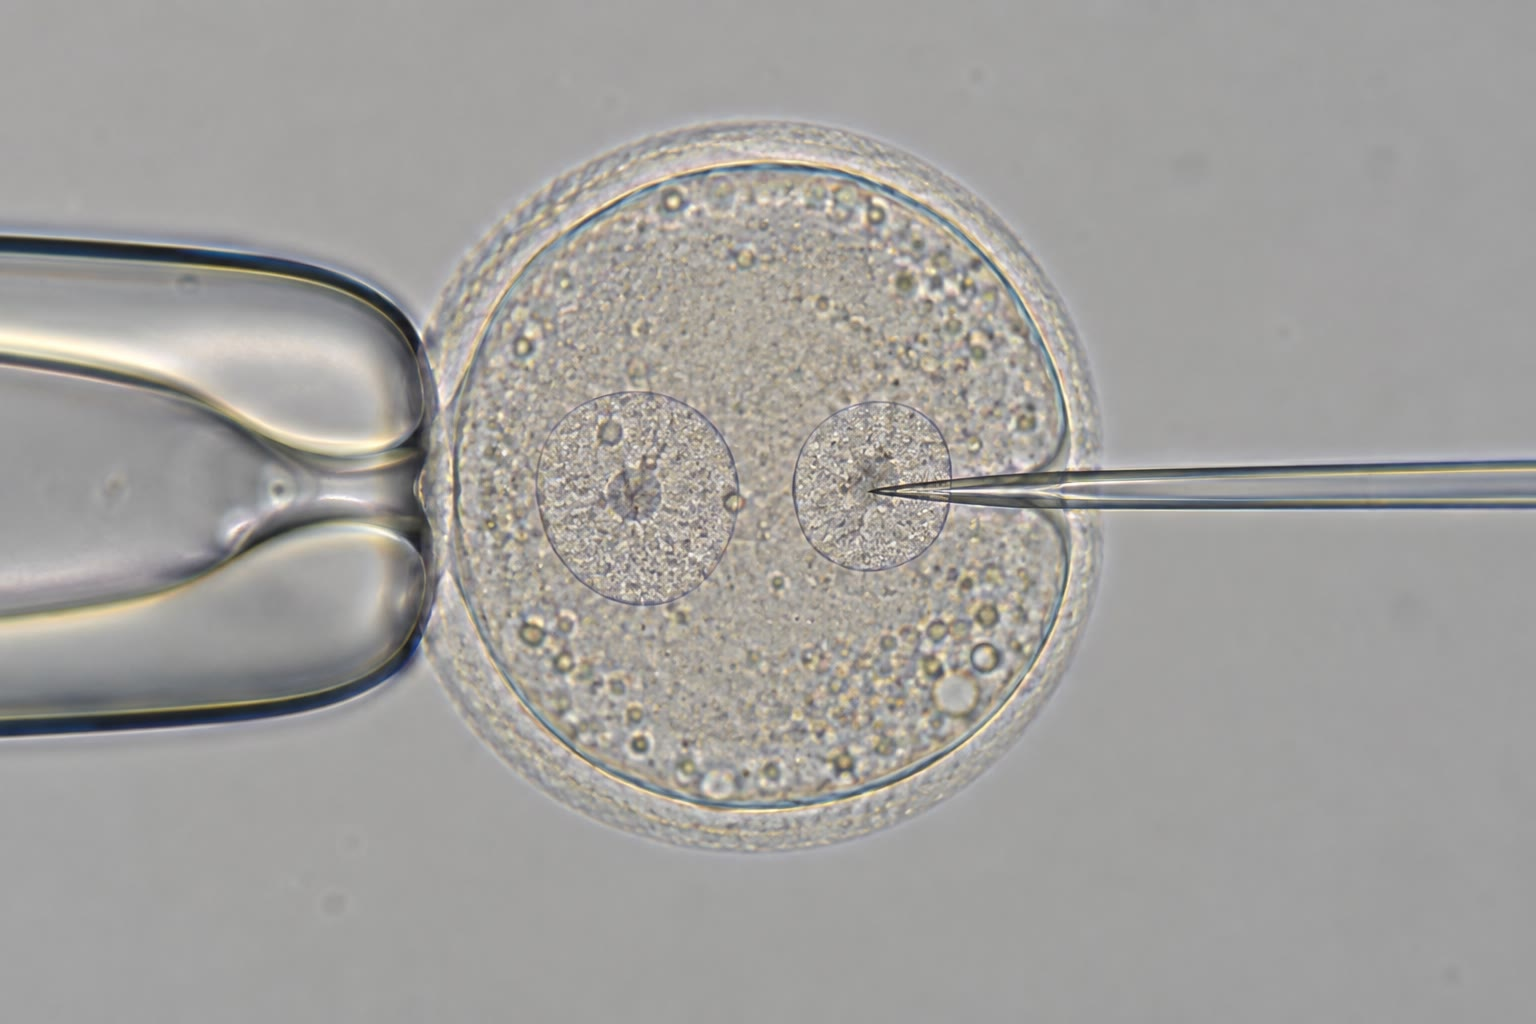
\includegraphics[width=0.46\linewidth]{images/book5/ai/b5-06-microinjection.jpg}\hspace{0.04\linewidth}
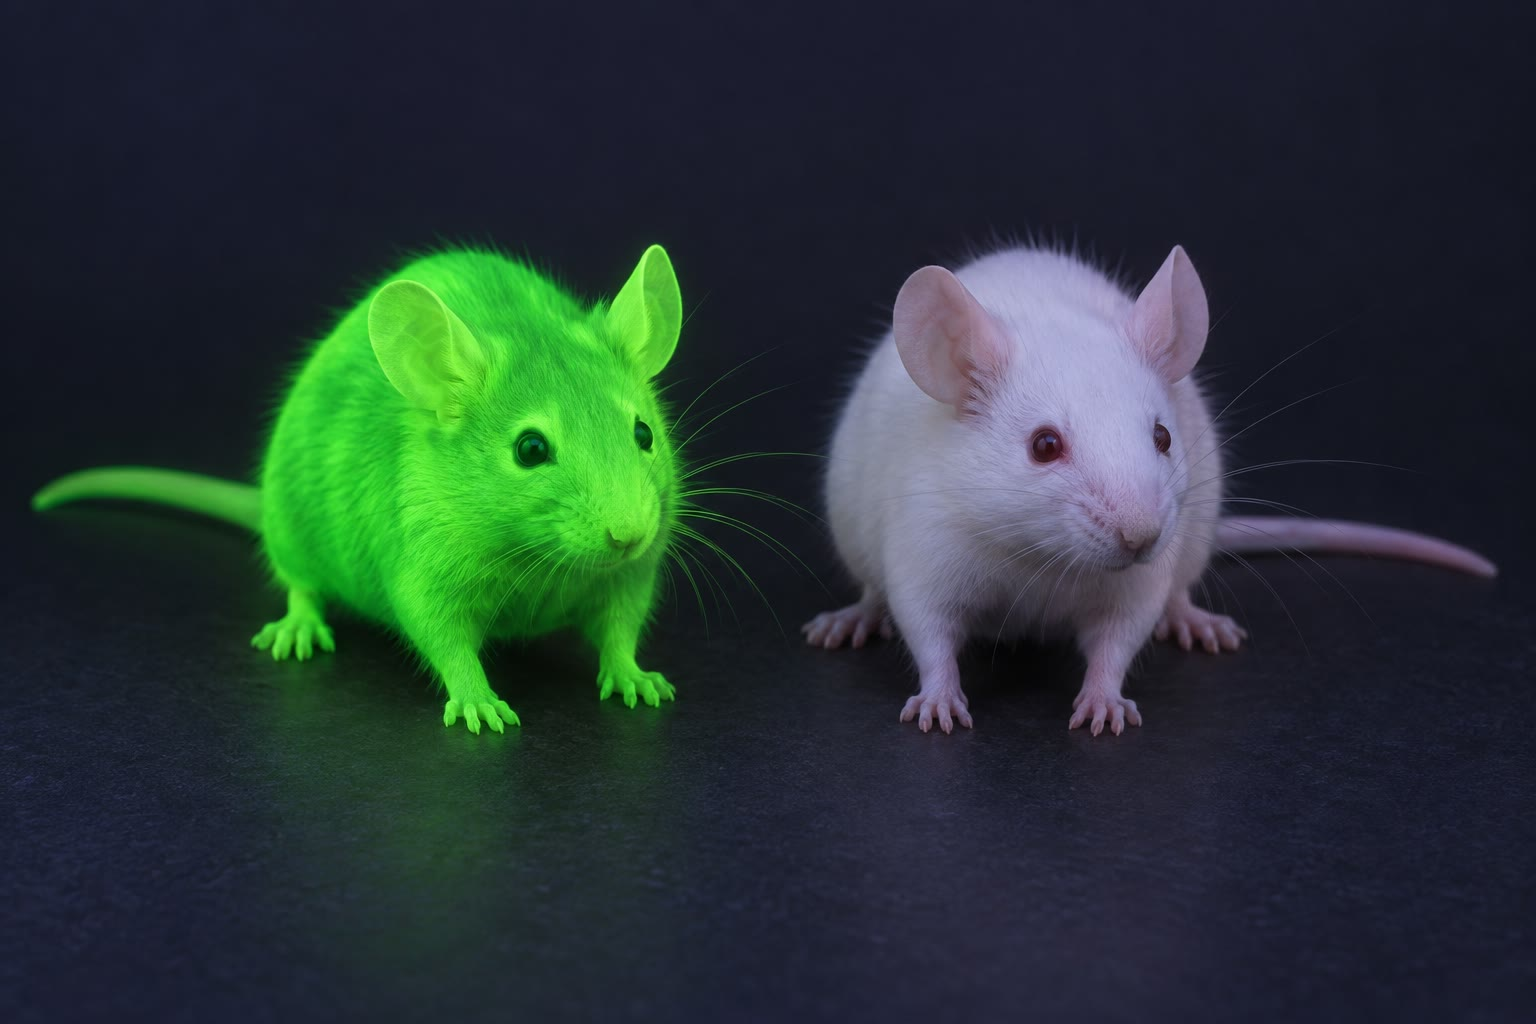
\includegraphics[width=0.46\linewidth]{images/book5/ai/b5-06-gfp-mouse.jpg}

{\small बाएँ: चूषण से थामा गया कोई निषेचित चूहा-अंडाणु, जबकि कोई काँच
की सुई एक पूर्वकेंद्रक में DNA अंतःक्षेपित कर रही है। दाएँ: हर कोशिका
में किसी जेलीफ़िश का हरा प्रतिदीप्त प्रोटीन अभिव्यक्त करता कोई \omterm{def:b3:genetic-engineering:transgenic}{पारजीनी}
चूहा, पराबैंगनी प्रकाश के नीचे किसी साधारण सहोदर के बगल में।}
\end{omfigure}

\begin{definition}[पारजीनी पौधे]\label{def:b3:genetic-engineering:plants}
\index{Agrobacterium}\index{T-DNA}\index{आनुवंशिक रूपांतरित फ़सल}
पौधों का रूपांतरण \emph{Agrobacterium tumefaciens} से होता है, जो
मिट्टी का ऐसा जीवाणु है जो स्वाभाविक रूप से अपने अर्बुद-प्रेरक
\omterm{def:b3:genetic-engineering:tools}{प्लाज़्मिड} का एक खंड, \emph{T-DNA}, किसी घायल पौधे के जीनोम में डाल देता
है ताकि पौधा कोई गाँठ उगाए और जीवाणु को खिलाए। T-DNA के अपने जीनों को
किसी भी चुने जीन से बदल देना, उन्हीं सीमा-अनुक्रमों के बीच जिन्हें
जीवाणु पहचानता है, रोगजनक को एक \omterm{def:b3:genetic-engineering:tools}{संवाहक} बना देता है; रूपांतरित कोशिकाएँ
चुनी जाती हैं और पूरे पौधों में पुनर्जनित की जाती हैं, जो हर पादप
कोशिका कर सकती है। जिन जातियों को यह जीवाणु संक्रमित नहीं करता (बहुत
समय तक अनाज) उनका रूपांतरण DNA-लेपित सोने के कणों को ऊतक में दागकर होता
है। बड़े पैमाने पर उगाई जाने वाली \emph{आनुवंशिक रूपांतरित फ़सलें}
कीट-डिंभों के विरुद्ध कोई जीवाणु विष जीन (\emph{Bt}) ढोती हैं, या कोई
जीवाणु एंज़ाइम जो किसी खरपतवारनाशी के प्रति सहिष्णुता देता है, या
दोनों; \emph{स्वर्ण चावल} कैरोटीनॉयड पथ के दो जीन ढोता है (कोई पादप
फ़ाइटोईन सिंथेज़ और कोई जीवाणु डीसैचुरेज़) ताकि उसका भ्रूणपोष
$\beta$-कैरोटीन बनाए, जो विटामिन~A का पूर्वगामी है और जिसकी कमी हर वर्ष
कई लाख बच्चों को अंधा करती और मारती है।
\end{definition}

\begin{omfigure}
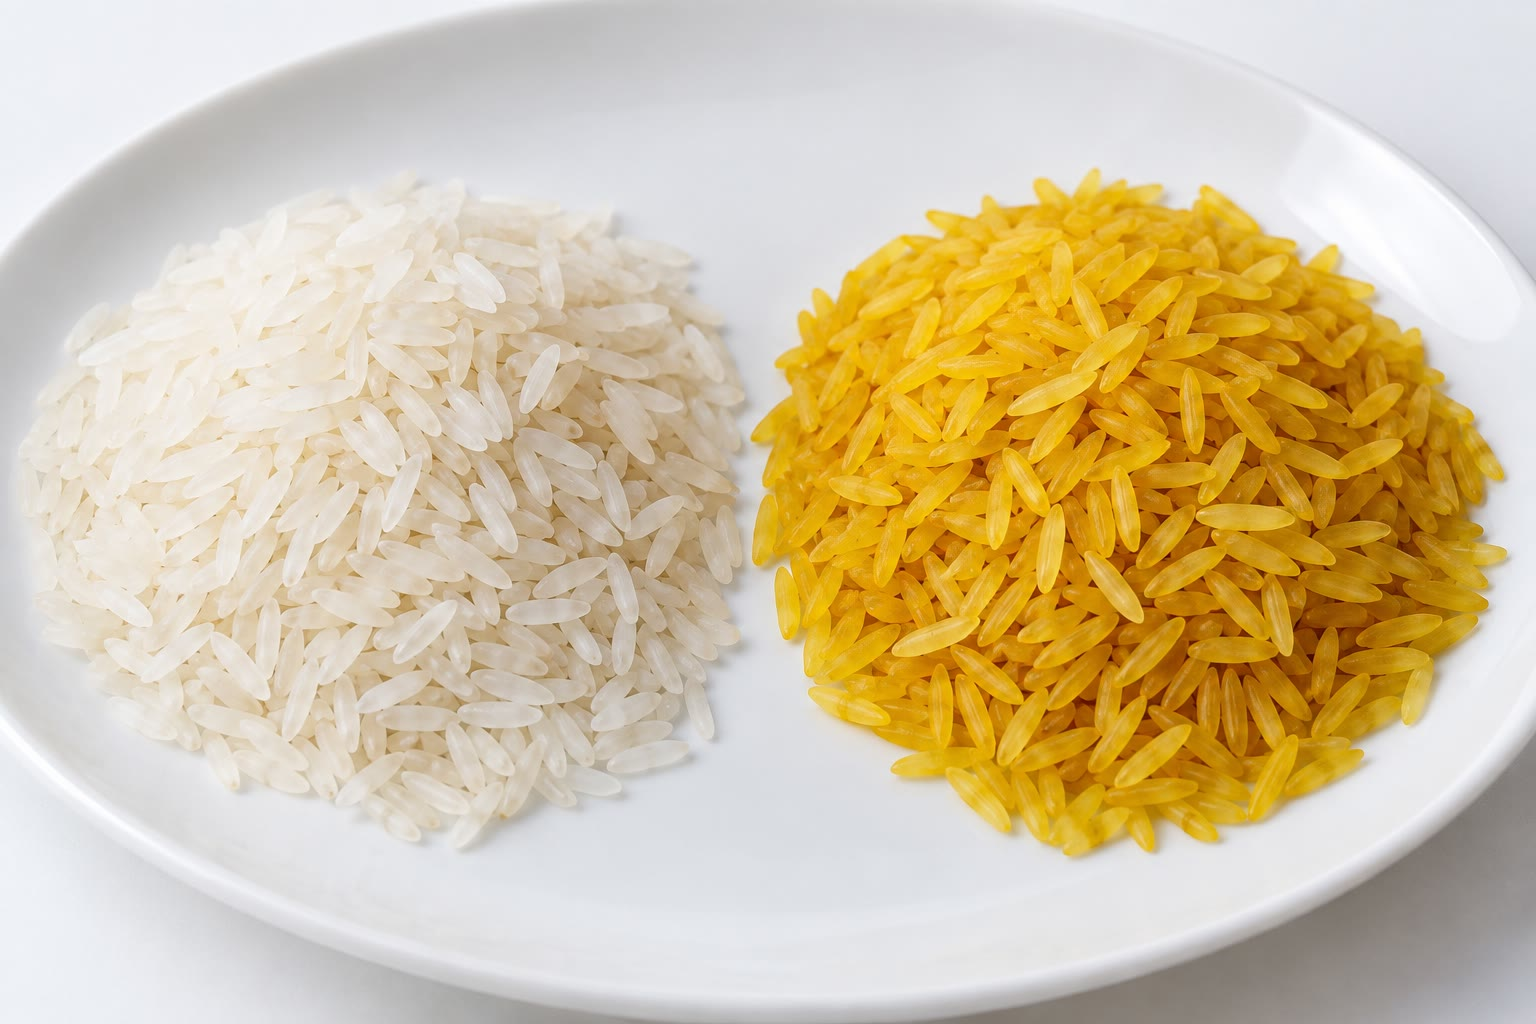
\includegraphics[width=0.46\linewidth]{images/book5/ai/b5-06-golden-rice.jpg}\hspace{0.04\linewidth}
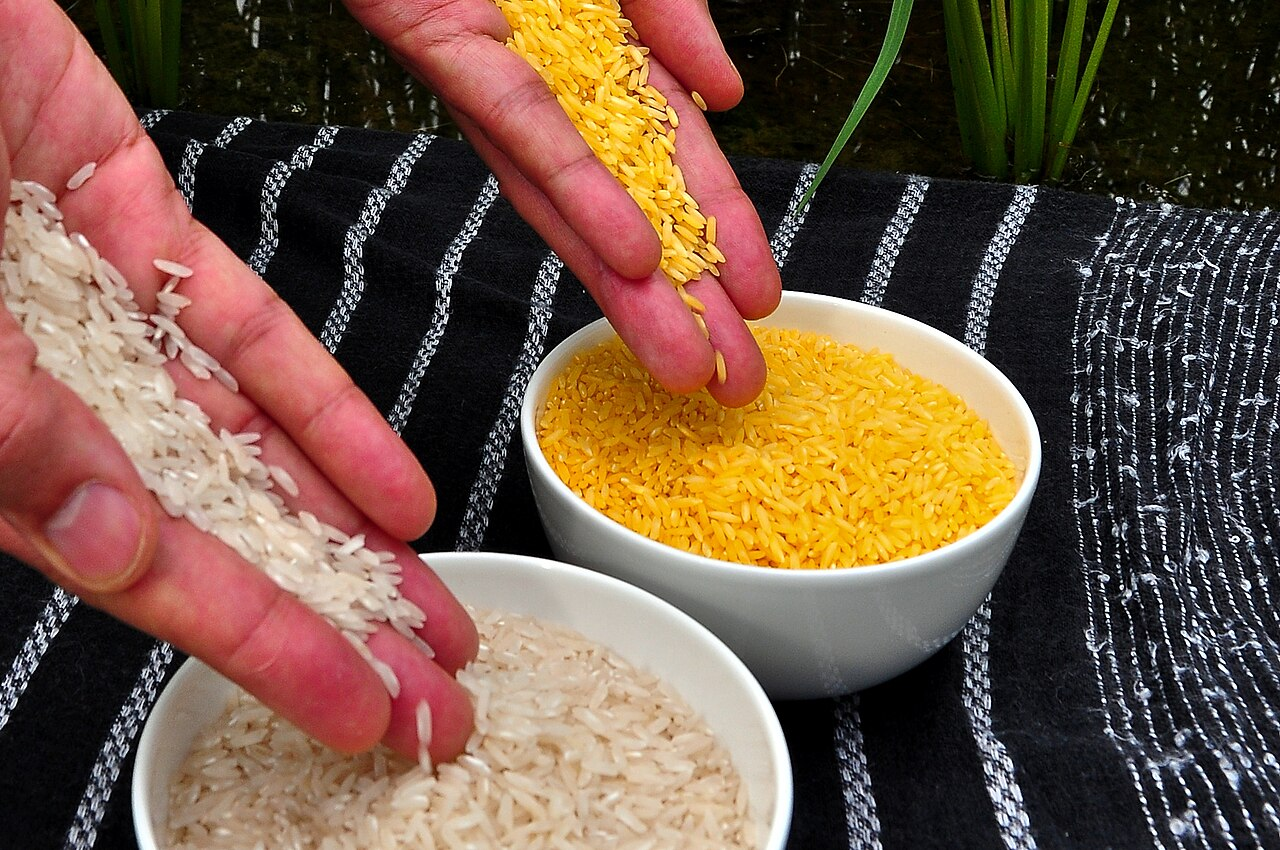
\includegraphics[width=0.46\linewidth]{images/book5/golden-rice-irri.jpg}

{\small साधारण और स्वर्ण चावल। पीला दाना अपने भ्रूणपोष में कैरोटीनॉयड
पथ के दो जोड़े गए जीनों से $\beta$-कैरोटीन बनाता है। दाएँ: दोनों चावल
अंतरराष्ट्रीय चावल अनुसंधान संस्थान (IRRI, CC~BY~2.0) में तुलना में।}
\end{omfigure}

\begin{remark}[बहस]\label{rem:b3:genetic-engineering:gmo}
करोड़ों हेक्टेयर पर तीस वर्षों की खेती, और वैज्ञानिक अकादमियों की हर
व्यवस्थित समीक्षा, में स्वीकृत \omterm{def:b3:genetic-engineering:transgenic}{पारजीनी} फ़सलों का ऐसा कोई स्वास्थ्य
प्रभाव नहीं मिला जो उनके परंपरागत समकक्षों से भिन्न हो; पारजीन चालीस
हज़ार में एक और जीन है, और वह जो प्रोटीन बनाता है उसकी जाँच किसी भी
खाद्य योजक की तरह होती है। असली प्रश्न पारिस्थितिक और आर्थिक हैं:
एकरूप चयन के अंतर्गत नाशीजीवों तथा खरपतवारों में प्रतिरोध का फैलना,
वन्य संबंधियों में जीन-प्रवाह, बीज-बाज़ार का संकेंद्रण, और लाभ किसे
मिलता है। ये वही प्रश्न हैं जो कोई भी सामर्थ्यवान कृषि-प्रौद्योगिकी
उठाती है, और उत्तर उस लक्षण और उस परिवेश पर निर्भर करते हैं, न कि उस
विधि पर जिससे जीन खिसकाया गया।
\end{remark}

\section{जीनोम संपादित करना}

\begin{definition}[CRISPR--Cas9]\label{def:b3:genetic-engineering:crispr}
\index{CRISPR}\index{Cas9}\index{मार्गदर्शक RNA}\index{PAM}\index{जीनोम संपादन}
जीवाणु उन फ़ेजों के जीनोमों के खंड, जिन्होंने उनके पूर्वजों को संक्रमित
किया था, पुनरावृत्तियों की किसी शृंखला (\emph{CRISPR}) में सँजोकर रखते
हैं, उनका अनुलेखन छोटे मार्गदर्शक RNA में करते हैं, और उनसे किसी
न्यूक्लिएज़ को यह निर्देश देते हैं कि कोशिका में घुसने वाला कोई भी मेल
खाता DNA काट दे: आनुवंशिक स्मृति वाली एक अनुकूली प्रतिरक्षा-प्रणाली।
\emph{Streptococcus pyogenes} में यह न्यूक्लिएज़ अकेला प्रोटीन
\emph{Cas9} है, जो किसी मार्गदर्शक RNA और किसी दूसरे छोटे RNA से बँधता
है, DNA में किसी तीन-क्षार \emph{प्रोटोस्पेसर-सन्निकट \omterm{def:b3:bioinformatics:motif}{अभिप्ररूप}}
(PAM, 5$'$-NGG) की खोज करता है, सटे DNA को खोलता है, और यदि PAM के पास
के बीस क्षार मार्गदर्शक से युग्मित हों तो PAM से तीन क्षार दूर दोनों
लड़ियाँ काट देता है। जिनेक, शार्पान्त्ये, डूडना और सहयोगियों (2012) ने
दोनों RNA को एक \emph{एकल-मार्गदर्शक RNA} में संलयित किया और दिखाया कि
किसी भी चुने अनुक्रम के मार्गदर्शक वाला Cas9 किसी परखनली में DNA को
उसी अनुक्रम पर काटता है; एक वर्ष के भीतर यह जोड़ी मानव, चूहा,
ज़ेब्राफ़िश, पादप और खमीर कोशिकाओं में काम करती दिखा दी गई। कटाव के
साथ कोशिका जो करती है वही \emph{जीनोम संपादन} है
सिरा-संयोजन कोई छोटा अंतर्वेशन या विलोपन छोड़ जाता है जो जीन को तोड़
देता है (एक ही चरण में, किसी भी जीव में, हफ़्तों में कोई \omterm{def:b3:genetic-engineering:transgenic}{निष्क्रियण}),
और दिए गए किसी साँचे के साथ \omterm{def:b3:dna-repair:dsb}{समजात पुनर्संयोजन} कोई चुना हुआ अनुक्रम लिख
देता है।
\end{definition}

\begin{omfigure}
\begin{tikzpicture}[every node/.style={font=\scriptsize}, >=stealth]
  % Cas9 outline (drawn first so labels stay on top)
  \draw[thick, omExo, fill=omExo!15] (5.9,1.1) ellipse (2.6 and 1.6);
  \node[omExo!60!black] at (7.7,2.3) {Cas9};
  % target DNA
  \draw[very thick, omDef] (0,0.3) -- (11,0.3); \draw[very thick, omDef] (0,-0.1) -- (11,-0.1);
  % PAM
  \fill[omProp!60] (7.2,-0.2) rectangle (7.9,0.4); \node[below] at (7.55,-0.25) {PAM (NGG)};
  % protospacer
  \draw[omThm, very thick] (4.2,0.5) -- (7.15,0.5); \node[above] at (5.7,0.55) {20-क्षार लक्ष्य, मार्गदर्शक से युग्मित};
  % guide RNA
  \draw[very thick, omMeth!70!black] (4.2,0.3) .. controls (4.2,1.6) and (5.0,1.9) .. (5.4,1.9) -- (6.6,1.9) .. controls (7.0,1.9) and (7.2,2.5) .. (6.8,2.8) .. controls (6.3,3.1) and (5.8,2.7) .. (6.1,2.4);
  \node[left, omMeth!70!black, align=right] at (3.2,2.2) {एकल-मार्गदर्शक RNA:\\चुने हुए 20 क्षार\\+ Cas9-बंधक हेयरपिन};
  % cut
  \draw[omThm, very thick, ->] (6.25,-0.7) -- (6.25,0.35); \node[omThm, below] at (6.25,-0.7) {द्विलड़ी विखंडन, PAM से 3 क्षार दूर};
  % outcomes
  \draw[->, thick] (2.0,-1.3) -- (2.0,-1.9); \node[below, align=center] at (2.0,-1.9) {सिरा-संयोजन:\\छोटा अंतर्वेशन या विलोपन\\$\Rightarrow$ ढाँचा-विस्थापन, निष्क्रियण};
  \draw[->, thick] (10.0,-1.3) -- (10.0,-1.9); \node[below, align=center] at (10.0,-1.9) {दिए गए साँचे के साथ\\पुनर्संयोजन\\$\Rightarrow$ परिशुद्ध बदलाव};
\end{tikzpicture}

{\small \omterm{def:b3:genetic-engineering:crispr}{Cas9} और उसका मार्गदर्शक। प्रोटीन किसी \omterm{def:b3:genetic-engineering:crispr}{PAM} से बँधता है, उसके पास
का DNA खोलता है, और यदि बीस क्षार \omterm{def:b3:genetic-engineering:crispr}{मार्गदर्शक RNA} से युग्मित हों तो काट
देता है। विखंडन की मरम्मत या तो सिरा-संयोजन से होती है, जो जीन तोड़
देता है, या किसी साँचे के साथ पुनर्संयोजन से, जो उसे फिर से लिख देता है।}
\end{omfigure}

\begin{proposition}[बिना विखंडन के संपादन]\label{prop:b3:genetic-engineering:editors}
\index{क्षार संपादक}\index{प्राइम संपादक}\index{लक्ष्येतर}
दोनों लड़ियाँ काटना सबसे भोंडा संपादन है: सिरा-संयोजन का परिणाम
यादृच्छिक होता है, और कहीं और पड़ा कोई विखंडन --- कोई \emph{लक्ष्येतर}
स्थल जो मार्गदर्शक से कुछ स्थितियों पर भिन्न हो और जिसे \omterm{def:b3:genetic-engineering:crispr}{Cas9} सह लेता है
--- ऐसा उत्परिवर्तन है जो किसी ने माँगा नहीं था। जिस \omterm{def:b3:genetic-engineering:crispr}{Cas9} का एक
न्यूक्लिएज़ प्रांत निष्क्रिय हो वह एक ही लड़ी में कटान लगाती है; दोनों
निष्क्रिय हों तो वह केवल बँधती है, और दूसरे एंज़ाइमों को किसी अनुक्रम
तक ले जा सकती है। \emph{\omterm{prop:b3:genetic-engineering:editors}{क्षार संपादक}} कटान लगाती \omterm{def:b3:genetic-engineering:crispr}{Cas9} को ऐसी
डीएमिनेज़ से संलयित करते हैं जो खुली लड़ी में C को U (जो T पढ़ा जाता
है) या A को I (जो G पढ़ा जाता है) में बदल देती है, और यह बिना किसी
विखंडन और बिना किसी साँचे के एक क्षार बदल देता है; \emph{\omterm{prop:b3:genetic-engineering:editors}{प्राइम संपादक}}
कोई प्रतिलोम अनुलेखक और वांछित अनुक्रम से बढ़ाया गया कोई मार्गदर्शक
ढोते हैं, और उस अनुक्रम की नकल कटान लगी लड़ी में कर देते हैं, जिससे कोई
भी प्रतिस्थापन और छोटे अंतर्वेशन या विलोपन संभव हो जाते हैं।
लक्ष्येतर क्रियाशीलता अभियंत्रित उच्च-निष्ठा \omterm{def:b3:genetic-engineering:crispr}{Cas9} रूपांतरों से,
एंज़ाइम को जीन के बजाय प्रोटीन के रूप में थोड़ी देर पहुँचाने से, और ऐसे
मार्गदर्शक चुनने से घटाई जाती है जिनके निकटतम जीनोमी संबंधी कई
स्थितियों पर भिन्न हों; उसका मापन पूर्वानुमानित स्थलों के अनुक्रमण से,
और ऐसी निष्पक्ष विधियों से होता है जो जीनोम का हर विखंडन पकड़ लेती हैं।
\end{proposition}

\begin{example}[एक इलाज]\label{ex:b3:genetic-engineering:sickle}
दात्र-कोशिका रोग $\beta$-ग्लोबिन में एक ही क्षार का बदलाव है।
$\gamma$-ग्लोबिन से बना भ्रूणीय हीमोग्लोबिन उसकी जगह ले सकता था, पर
$\gamma$ जीन जन्म के बाद दमनकारी BCL11A द्वारा बंद कर दिए जाते हैं।
पहली स्वीकृत \omterm{def:b3:genetic-engineering:crispr}{CRISPR} चिकित्सा (2023) रोगी की अपनी रक्त-स्तंभ कोशिकाएँ
लेती है, \emph{BCL11A} के रक्ताणु संवर्धक को \omterm{def:b3:genetic-engineering:crispr}{Cas9} से काटती है ताकि
सिरा-संयोजन उसे अधिकांश कोशिकाओं में निष्क्रिय कर दे, और रोगी की मज्जा
साफ़ कर देने के बाद कोशिकाएँ लौटा देती है: वे जो लाल कोशिकाएँ बनाती हैं
वे भ्रूणीय हीमोग्लोबिन से भरपूर होती हैं, दात्राकार नहीं होतीं, और
संकट रुक जाते हैं। यह संपादन कायिक है --- जनन-वंश अछूता रहता है और
बदलाव वंशागत नहीं होता --- और वह ``भोंडा'' परिणाम, यानी तोड़ना, वहीं
काम में लेता है जहाँ तोड़ना ही चाहिए।
\end{example}

\begin{theorem}[किसी जीन-चालक का अति-मेंडेली फैलाव]\label{thm:b3:genetic-engineering:drive}
\index{जीन-चालक}
कोई \emph{\omterm{thm:b3:genetic-engineering:drive}{जीन-चालक}} ऐसी रचना है जो \omterm{def:b3:genetic-engineering:crispr}{Cas9} और ऐसे मार्गदर्शक का कूटलेखन
करती है जो किसी विषमयुग्मजी में अपने ही स्थल पर वन्य-प्ररूप
युग्मविकल्पी को काट देता है; पुनर्संयोजन से मरम्मत चालक की नकल कटे
गुणसूत्र में उतार देती है, जिससे मेंडेली आधे के बजाय विषमयुग्मजी के
युग्मकों का कोई अंश $c$ चालक ढोता है। यदि किसी बड़ी, यादृच्छिक रूप से
संगम करती समष्टि में चालक की बारंबारता $p$ हो और कोई अनुकूलता-लागत न
हो, तो अगली पीढ़ी में उसकी बारंबारता है
\[
p' = p + c\,p\,(1 - p),
\]
इसलिए वह दुर्लभता से $c$ के समानुपाती दर से फैलता है, और लगभग
$\ln(1/p_{0})/\ln(1 + c)$ पीढ़ियों में आधी समष्टि तक पहुँच जाता है,
जब आरंभिक बारंबारता $p_{0}$ हो।
\end{theorem}
\begin{proof}
यादृच्छिक संगम चालक के समयुग्मजी बारंबारता $p^{2}$ पर देता है,
विषमयुग्मजी $2p(1-p)$ पर, वन्य-प्ररूप समयुग्मजी $(1-p)^{2}$ पर।
समयुग्मजी चालक अपने सारे युग्मकों को देते हैं, विषमयुग्मजी
$(1 + c)/2$ अंश को (आधा मेंडेल से, और $c$ गुना वन्य-प्ररूप आधा
रूपांतरित), वन्य-प्ररूप किसी को नहीं। इसलिए $p' = p^{2} + 2p(1-p)(1+c)/2
= p^{2} + p(1-p) + c\,p(1-p) = p + c\,p(1-p)$। छोटे $p$ के लिए यह
$p' \approx (1+c)p$ है, यानी अनुपात $1 + c$ से गुणोत्तर वृद्धि, जो
$1/2$ तक पहुँचती है, $p_{0}$ से लगभग $\ln(1/2p_{0})/\ln(1+c)$ पीढ़ियों
में; संभार्य पद उसे केवल अंत के पास धीमा करता है।
\end{proof}

\begin{omfigure}
\begin{tikzpicture}
\begin{axis}[
  width=0.7\linewidth, height=5.6cm,
  axis x line=bottom, axis y line=left,
  xmin=0, xmax=20, ymin=0, ymax=1.05,
  xlabel={पीढ़ी}, ylabel={चालक बारंबारता $p$},
  xlabel style={font=\small, at={(axis description cs:0.5,-0.12)}, anchor=north},
  ylabel style={font=\small},
  tick label style={font=\small}, xtick={0,5,10,15,20}, ytick={0,0.5,1},
  clip=false,
]
\addplot[very thick, omThm, mark=*, mark size=1.2pt] coordinates {(0,0.01) (1,0.0189) (2,0.0356) (3,0.0665) (4,0.1224) (5,0.2191) (6,0.3731) (7,0.5836) (8,0.8023) (9,0.9451) (10,0.9918) (11,0.9991) (12,1.0) (13,1.0) (14,1.0) (15,1.0) (16,1.0) (17,1.0) (18,1.0) (19,1.0) (20,1.0)};
\addplot[very thick, omDef, mark=*, mark size=1.2pt] coordinates {(0,0.01) (1,0.015) (2,0.0223) (3,0.0332) (4,0.0493) (5,0.0727) (6,0.1064) (7,0.154) (8,0.2191) (9,0.3047) (10,0.4106) (11,0.5316) (12,0.6561) (13,0.769) (14,0.8578) (15,0.9188) (16,0.9561) (17,0.9771) (18,0.9883) (19,0.9941) (20,0.997)};
\addplot[very thick, gray, dashed, domain=0:20, samples=2] {0.01};
\node[font=\scriptsize, omThm, anchor=south east] at (axis cs:6.5,0.62) {$c = 0.9$};
\node[font=\scriptsize, omDef, anchor=north west] at (axis cs:12.5,0.62) {$c = 0.5$};
\node[font=\scriptsize, gray, anchor=south west] at (axis cs:12,0.02) {मेंडेली, $c = 0$: $p_{0}$ पर ही रहता है};
\end{axis}
\end{tikzpicture}

{\small एक प्रतिशत पर छोड़ा गया कोई \omterm{thm:b3:genetic-engineering:drive}{जीन-चालक}, रूपांतरण-दक्षता
$0.9$ या $0.5$ और बिना किसी अनुकूलता-लागत के। बिना किसी लाभ वाला कोई
मेंडेली युग्मविकल्पी एक प्रतिशत पर ही रहता; चालक दस या बीस पीढ़ियों
में छा जाता है।}
\end{omfigure}

\begin{remark}[क्या संपादित किया जा सकता है]\label{rem:b3:genetic-engineering:ethics}
किसी सहमत रोगी की कायिक कोशिकाओं का संपादन चिकित्सा है, जिसे किसी भी
उपचार की तरह उसके जोखिमों और लाभों से परखा जाता है। जनन-वंश का संपादन
--- किसी भ्रूण का, जिसका हर वंशज वह बदलाव ढोएगा --- प्रकार से ही भिन्न
है: जो व्यक्ति प्रभावित होगा वह सहमति नहीं दे सकता, बदलाव वंशागत होता
है, और तकनीक के लक्ष्येतर तथा विचित्र परिणाम अभी नियंत्रित नहीं हैं;
2018 में एक चीनी वैज्ञानिक द्वारा जुड़वाँ बच्चों में ऐसा करने की घोषणा
के बाद अधिकांश देशों की वैज्ञानिक अकादमियों ने रोक की माँग की और कई
राज्यों ने उसे अपराध बना दिया। किसी वन्य समष्टि में छोड़ा गया कोई
\omterm{thm:b3:genetic-engineering:drive}{जीन-चालक} ऐसा निर्णय है जो आगे आने वाले सबके लिए लिया जाता है, इसीलिए
मलेरिया-मच्छरों को समाप्त करने के लिए इसी क्षेत्र के अपने प्रस्ताव
चालकों को विफलता-सुरक्षाओं से --- उलटने वाले चालक, स्वयं-सीमित अभिकल्प
--- और संबंधित देशों की सार्वजनिक सहमति से जोड़ते हैं।
\end{remark}

\section{अभ्यास}

\begin{exercise}[$\star$]\label{exo:b3:genetic-engineering:1}
किसी क्लोनन \omterm{def:b3:genetic-engineering:tools}{प्लाज़्मिड} में जो तीन अंग होने चाहिए उन्हें गिनाइए और हर एक
का प्रयोजन समझाइए।
\end{exercise}

\begin{exercise}[$\star$]\label{exo:b3:genetic-engineering:2}
EcoRI GAATTC को पहचानती है। यादृच्छिक DNA में यह स्थल औसतन कितनी बार
आता है, और \qty{4.6}{Mb} के \emph{E.~coli} जीनोम के वह कितने खंड बनाती
है? असली संख्या कुछ भिन्न क्यों है?
\end{exercise}

\begin{exercise}[$\star$]\label{exo:b3:genetic-engineering:3}
किसी PCR चक्र के तीन ताप-चरण और हर एक पर क्या होता है, बताइए।
पॉलीमरेज़ का ताप-स्थायी होना क्यों आवश्यक है?
\end{exercise}

\begin{exercise}[$\star$]\label{exo:b3:genetic-engineering:4}
किसी दिए हुए अनुक्रम को काटने के लिए \omterm{def:b3:genetic-engineering:crispr}{Cas9} को क्या चाहिए, और कटाव के
बाद कौन-से दो परिणाम हो सकते हैं?
\end{exercise}

\begin{exercise}[$\star\star$]\label{exo:b3:genetic-engineering:5}
कोई PCR $35$ चक्र दक्षता $E = 0.9$ पर $50$ प्रतियों से चलती है। कितनी
प्रतियाँ मिलती हैं? दो प्रतिदर्शों की qPCR $C_{T} = 18.2$ और $25.5$
देती है; $E = 0.95$ के साथ उनकी आरंभिक मात्राओं का अनुपात क्या है?
\end{exercise}

\begin{exercise}[$\star\star$]\label{exo:b3:genetic-engineering:6}
जीवाणुओं में किसी मानव प्रोटीन की अभिव्यक्ति के लिए कोई cDNA संचय काम
में आता है, कोई जीनोमी संचय क्यों नहीं? \emph{E.~coli} में कोई मानव
प्रोटीन बनाने की दो और अड़चनें बताइए और हर एक को कैसे पार किया जाता है।
\end{exercise}

\begin{exercise}[$\star\star$]\label{exo:b3:genetic-engineering:7}
\omterm{def:b3:genetic-engineering:transgenic}{भ्रूणीय स्तंभ कोशिकाओं} में \omterm{def:b3:genetic-engineering:transgenic}{जीन-लक्ष्यन} से कोई निष्क्रियण-चूहा बनाया
जाता है। समझाइए कि जन्मा पहला चूहा विचित्रकाय क्यों होता है, उसका
प्रजनन क्यों करना पड़ता है, और यदि किसी ऐसे विचित्रकाय के, जिसका
जनन-वंश आधा लक्षित है, विषमयुग्मजी नाती-पोतों का अंतःसंकरण कराया जाए तो
उसके नाती-पोतों का कितना अंश समयुग्मजी \omterm{def:b3:genetic-engineering:transgenic}{निष्क्रियण} होगा।
\end{exercise}

\begin{exercise}[$\star\star$]\label{exo:b3:genetic-engineering:8}
NGG \omterm{def:b3:genetic-engineering:crispr}{PAM} वाला 20 क्षारों का कोई \omterm{def:b3:genetic-engineering:crispr}{मार्गदर्शक RNA} चुना जाता है।
$3.2\times 10^{9}$ bp के किसी जीनोम में (दोनों लड़ियाँ) संयोग से कितने
स्थल मार्गदर्शक से ठीक-ठीक मेल खाएँगे? यदि \omterm{def:b3:genetic-engineering:crispr}{Cas9} दो तक असंगतियाँ सह ले
तो कितने मेल खाएँगे? (दो असंगतियों के भीतर के अनुक्रम $1 + 3\binom{20}{1} +
9\binom{20}{2}$ गिनिए।)
\end{exercise}

\begin{exercise}[$\star\star$]\label{exo:b3:genetic-engineering:9}
\cref{thm:b3:genetic-engineering:drive} का उपयोग करते हुए
$c = 0.8$ वाले किसी चालक की बारंबारता $p_{0} = 0.05$ से तीन पीढ़ियों के
बाद निकालिए, और $0.5$ तक पहुँचने में लगने वाली पीढ़ियों का आकलन कीजिए।
\end{exercise}

\begin{exercise}[$\star\star\star$]\label{exo:b3:genetic-engineering:10}
दात्र-कोशिका चिकित्सा $\beta$-ग्लोबिन उत्परिवर्तन को सुधारने के बजाय
किसी संवर्धक को तोड़ती है। रक्त-स्तंभ कोशिकाओं में \omterm{def:b3:dna-repair:dsb}{समजात पुनर्संयोजन}
से सुधार के बजाय सिरा-संयोजन से तोड़ना क्यों चुना गया, इसके दो कारण
दीजिए, और एक हानि भी।
\end{exercise}

\begin{exercise}[$\star\star\star$]\label{exo:b3:genetic-engineering:11}
किसी मच्छर के विरुद्ध कोई \omterm{thm:b3:genetic-engineering:drive}{जीन-चालक} समयुग्मजियों में अनुकूलता-लागत $s$
ढोता है। चालक-समयुग्मजियों के विरुद्ध चयन को समाविष्ट करने के लिए
पुनरावृत्ति-संबंध बदलिए और चालक के दुर्लभता से फैलने के लिए $c$ तथा
$s$ पर प्रतिबंध ढूँढ़िए। फिर समझाइए कि व्यवहार में प्रतिरोध
युग्मविकल्पी --- लक्ष्य पर बने वे सिरा-संयोजन उत्पाद जिन्हें मार्गदर्शक
अब नहीं पहचानता --- मुख्य बाधा क्यों हैं।
\end{exercise}

\begin{exercise}[$\star\star\star$]\label{exo:b3:genetic-engineering:12}
इस अध्याय की और \cref{ch:b3:dna-repair} की क्रियाविधियों से तर्क दीजिए
कि किसी मानव भ्रूण का जनन-वंश-संपादन अभी हर कोशिका में अभीष्ट परिणाम
की गारंटी क्यों नहीं दे सकता, और किसी विवेकी व्यक्ति के उसे सुरक्षित
मानने से पहले कौन-से प्रमाण चाहिए होंगे।
\end{exercise}

\section{समस्या: किसी जीन से एक औषध और एक फ़सल तक}

\begin{problem}[{सप्तांत समस्या --- प्रतिबंधन स्थलों तथा रूपांतरण के
अंकगणित से क्लोनित कोई जीन, qPCR से गिना गया कोई विषाणु, किसी किण्वक में
टन भर बनता कोई हॉर्मोन, लक्ष्येतर स्थलों की गिनती के साथ संपादित कोई
जीनोम, और समयबद्ध किया गया कोई जीन-चालक, जिसका अंत किसी प्रतिदर्श में
विषाणु की प्रतियों, संसार भर के इंसुलिन के लिए वार्षिक किण्वक-आयतन और
किसी चालक को चाहिए पीढ़ियों की संख्या पर होता है}]
\label{pb:b3:genetic-engineering:1}
आँकड़े: कोई \qty{1.5}{kb} जीन; कोई छह-क्षार प्रतिबंधन स्थल;
\qty{4}{kb} का कोई \omterm{def:b3:genetic-engineering:tools}{प्लाज़्मिड}; रूपांतरण दक्षता प्रति माइक्रोग्राम
\omterm{def:b3:genetic-engineering:tools}{प्लाज़्मिड} $2\times 10^{7}$ बस्तियाँ; जोड़ने से \qty{10}{\%} \omterm{def:b3:genetic-engineering:tools}{प्लाज़्मिडों}
को कोई अंतर्वेशन मिलता है। qPCR दक्षता $E = 1$, देहली $N_{T} = 10^{12}$।
इंसुलिन: \qty{5.8}{kDa}, कोई रोगी दिन में $40$ इकाई काम में लेता है, और
एक इकाई \qty{35}{\micro g} है; $10^{7}$ रोगी; कोई किण्वक प्रति बारी
\qty{2}{g/L} उत्पाद देता है, वर्ष में दस बारियाँ। जीनोम $3.2\times
10^{9}$ bp। चालक रूपांतरण $c = 0.9$, $p_{0} = 0.001$ पर छोड़ा गया।

\medskip
\noindent\textbf{भाग I --- क्लोनन।}
\begin{enumerate}
  \item यादृच्छिक DNA में कोई दिया हुआ छह-क्षार स्थल कितनी बार आता है?
        इसकी प्रायिकता क्या है कि \qty{1.5}{kb} जीन में ऐसा कोई स्थल
        न हो, ताकि एंज़ाइम से उसे पूरा क्लोनित किया जा सके?
  \item यदि उसमें कोई स्थल हो तो आप उसे फिर भी कैसे क्लोनित करेंगे?
        (दो विधियाँ।)
  \item जोड़े गए \omterm{def:b3:genetic-engineering:tools}{प्लाज़्मिड} का \qty{100}{ng} रूपांतरित किया जाता है।
        कितनी बस्तियाँ, और कितनी में अंतर्वेशन है?
  \item नीली--सफ़ेद छानबीन काम में ली जाती है। बस्तियों का कितना अंश
        सफ़ेद है, और \qty{99}{\%} संभावना के लिए कि कम-से-कम एक में
        जीन सही दिशा में हो (अंतर्वेशनों का आधा), कितनी सफ़ेद बस्तियाँ
        उठानी पड़ेंगी?
  \item पुनर्योगज \omterm{def:b3:genetic-engineering:tools}{प्लाज़्मिड} \qty{5.5}{kb} का है। कोई कोशिका $50$
        प्रतियाँ रखती है और हर \qty{30}{min} में विभाजित होती है। एक
        कोशिका से रात भर की वृद्धि (\qty{16}{h}) के बाद कितने
        \omterm{def:b3:genetic-engineering:tools}{प्लाज़्मिड} अणु, और \omterm{def:b3:genetic-engineering:tools}{प्लाज़्मिड} DNA का कितना द्रव्यमान
        (\qty{650}{Da} प्रति क्षार युग्म)?
  \item \omterm{def:b3:genetic-engineering:tools}{प्लाज़्मिड} को कोई जीवाणु उद्गम क्यों चाहिए, पर अंतर्वेशित मानव
        जीन को क्लोनन के लिए कोई जीवाणु प्रवर्तक नहीं चाहिए, जबकि
        अभिव्यक्ति के लिए चाहिए?
\end{enumerate}

\medskip
\noindent\textbf{भाग II --- कोई विषाणु गिनना।}
\begin{enumerate}[resume]
  \item किसी रोगी का प्रतिदर्श $C_{T} = 28$ पर देहली पार करता है।
        अभिक्रिया में कितनी प्रतियाँ थीं? $C_{T} = 35$ वाले दूसरे में?
  \item संवेदिता: किसी एक प्रति को देहली तक लाने में कितने चक्र लगते
        हैं?
  \item परीक्षण की कट-ऑफ़ $C_{T} = 38$ पर रखी गई है। वह कितनी
        प्रतियों के तुल्य है, और $45$ चक्र क्यों न रखें?
  \item किसी पिछली बारी के उत्पाद का कोई संदूषक अणु किसी ऋणात्मक
        प्रतिदर्श में घुस जाता है। वह किस चक्र पर देहली पार करेगा?
        कौन-सा प्रयोगशाला-व्यवहार इसे रोकता है?
  \item प्रतिलोम अनुलेखन विषाणु-RNA का \qty{40}{\%} DNA में बदलता है।
        पहले प्रतिदर्श के लिए प्रश्न 7 की गणना संशोधित कीजिए।
  \item दो प्रतिदर्श $\Delta C_{T} = 3.3$ से भिन्न हैं, $E = 1$ के
        साथ, पर दक्षता वस्तुतः $0.9$ है। विश्लेषक कितने गुने का अंतर
        बताता है, और सही अंतर क्या है?
\end{enumerate}

\medskip
\noindent\textbf{भाग III --- टन भर इंसुलिन।}
\begin{enumerate}[resume]
  \item प्रति रोगी दैनिक इंसुलिन-द्रव्यमान और $10^{7}$ रोगियों के लिए
        वार्षिक विश्व-आवश्यकता किलोग्राम में निकालिए।
  \item वह कितने मोल इंसुलिन हुआ, और कितने अणु?
  \item वर्ष में दस बारियाँ चलाने पर उसे कौन-सा किण्वक-आयतन बनाता है?
        \qty{2500}{m^3} के किसी तरण-ताल से तुलना कीजिए।
  \item ग्रंथियों से निष्कर्षण \qty{8000}{kg} अग्न्याशय से
        \qty{1}{kg} इंसुलिन देता था; किसी सूअर के अग्न्याशय का भार
        \qty{100}{g} है। संसार को वर्ष में कितने सूअर चाहिए होते?
  \item जहाँ पशु-इंसुलिन सस्ता है वहाँ भी पुनर्योगज हॉर्मोन को वरीयता
        क्यों दी जाती है? दो कारण दीजिए।
  \item इंसुलिन अनुरूप मानव अनुक्रम से एक-दो अवशेष भिन्न होते हैं।
        समझाइए कि कोई अनुरूप फिर भी ऐसी औषध क्यों है जो मानव ग्राही
        पर काम करती है, और एक अवशेष का बदलाव उसका वियोजन-काल क्यों
        बदल सकता है।
\end{enumerate}

\medskip
\noindent\textbf{भाग IV --- संपादन और चालन।}
\begin{enumerate}[resume]
  \item 20-क्षार मार्गदर्शक और NGG के कितने ठीक-ठीक मेल जीनोम में
        संयोग से हैं (दोनों लड़ियाँ: $6.4\times 10^{9}$
        स्थितियाँ)?
  \item यदि \omterm{def:b3:genetic-engineering:crispr}{Cas9} तीन तक असंगतियाँ सह ले, तो मार्गदर्शक से तीन
        असंगतियों के भीतर कितने अनुक्रम हैं, और इससे कितने संयोगी
        लक्ष्येतर स्थल बनते हैं?
  \item संपादित रक्त-स्तंभ कोशिकाएँ $10^{7}$ हैं; \qty{80}{\%} में
        अभीष्ट तोड़ हुआ है। यदि किसी दिए हुए स्थल पर $10^{4}$ में एक
        कोशिका कटती हो तो उस स्थल पर कितनी कोशिकाओं में लक्ष्येतर
        विखंडन है, और किसी एक स्तंभ कोशिका में किसी अर्बुद-दमनकारी जीन
        का विखंडन चिंता की बात क्यों है?
  \item चालक की बारंबारता $1, 2, 3$ पीढ़ियों के बाद
        $p_{0} = 0.001$ से निकालिए, और $0.5$ तक पीढ़ियों का आकलन कीजिए।
  \item किसी मच्छर की वर्ष में दस पीढ़ियाँ होती हैं। छा जाने में कितने
        वर्ष? समयुग्मजियों में \qty{20}{\%} की अनुकूलता-लागत चित्र को
        गुणात्मक रूप से कैसे बदल देती है?
  \item कोई प्रतिरोध युग्मविकल्पी तब उठता है जब कटाव की मरम्मत
        पुनर्संयोजन से नहीं, सिरा-संयोजन से हो, और यह प्रति
        रूपांतरण-प्रयास प्रायिकता $1 - c = 0.1$ से होता है। एक पीढ़ी
        में $10^{6}$ विषमयुग्मजियों की किसी समष्टि में बने प्रतिरोध
        युग्मविकल्पियों की संख्या आँकिए, और बताइए कि यदि वे अनुकूल
        हों तो चालक का क्या होता है।
  \item सारांश दीजिए: पहले प्रतिदर्श में प्रतियाँ (प्रश्न~7), संसार का
        वार्षिक इंसुलिन किण्वक-आयतन (प्रश्न~15), और चालक के आधी
        समष्टि तक पहुँचने की पीढ़ियाँ (प्रश्न~22)।
\end{enumerate}
\end{problem}
